\documentclass[11pt, oneside]{article} 
\usepackage{geometry}
\geometry{letterpaper} 
\usepackage{graphicx}
	
\usepackage{amssymb}
\usepackage{amsmath}
\usepackage{parskip}
\usepackage{color}
\usepackage{hyperref}

\graphicspath{{/Users/telliott_admin/Tex/png/}}
% \begin{center} 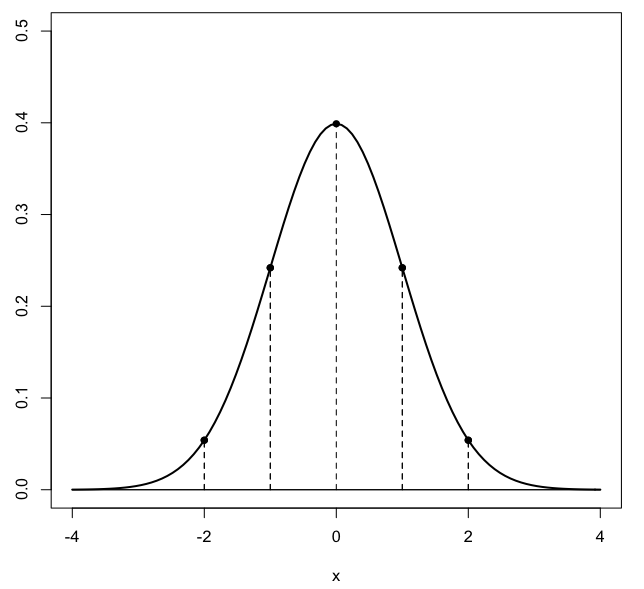
\includegraphics [scale=0.4] {gauss3.png} \end{center}

\title{First steps in calculus}
\date{}

\begin{document}
\maketitle
\Large

\hypertarget{first_calculus}{}
One example to appreciate the fundamental ideas in calculus is to refer to the instruments one uses while driving a car. Most drivers refer fairly often to the speedometer, which measures velocity, or "how fast you're going".

On the other hand, if someone wants to know about distance covered they might check the odometer.

\begin{center} 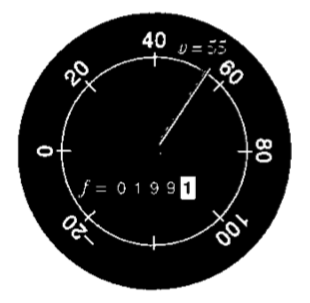
\includegraphics [scale=0.4] {Strang_speedometer.png} \end{center}

In calculus we say that the velocity is the \textbf{derivative} of the distance with respect to time, and the distance is the \textbf{integral} of the speed with respect to time.  The latter must be evaluated between starting and stopping points for the time, as we'll see.

(We can think of speed and velocity as the same for now.)

\subsection*{time-dependence}
Distance equals velocity times time.

This is easy if the velocity is a constant.  Travel at $60$ miles per hour for $2$ hours and you'll go $120$ miles.  It is standard to use $s$ to refer to the distance traveled and $v$ for velocity.  If the velocity is constant then:
\[ s = vt \]

Suppose we plot velocity as a \emph{function of time} ($v$ on the $y$-axis and $t$ on the $x$-axis).

If the velocity is constant, then we obtain a straight horizontal line.  Furthermore, the distance traveled is the \emph{area under the curve} (and above the $x$-axis) which is the area of a rectangle with sides $v$ and $t$ and as we said $s = vt$.

However, for many interesting problems velocity is not constant.  

For a car, imagine increasing the pressure on the gas pedal steadily so that, starting from a stop at zero time, after $1$ second you are going $10$ mph, after $2$ seconds $20$ mph, after $3$ seconds $30$ mph. If we continue at the same rate, we'll accelerate from $0$ to $60$ mph in $6$ seconds (quite a respectable time).

\begin{center} 
\includegraphics [scale=0.5] {Calc5_2.png} \end{center}

This is constant acceleration.

We say that $v$ is a constant function of time, and we can write 
\[ v = at \]

If acceleration is constant then $v$ changes with time.  If we start from $v=0$ then the final velocity will be $v = at$, but the distance traveled is not 
\[ s = vt \stackrel{?}{=} at^2 \]

Why not?

For variable velocity, the distance traveled is the \emph{average} velocity times the time.  For smooth acceleration from zero to $v$, the average velocity is
\[ v_{\text{avg}} = \frac{v}{2} \]

So the correct equation is:
\[ s = v_{\text{avg}}\ t = \frac{1}{2} at^2 \]

In this case, if we plot velocity as a function of time, we obtain a straight line that extends diagonally up with respect to the $x$-axis.  The distance traveled is the area under the curve (below the line and above the $x$-axis).  

The shape whose area is needed is a triangle.  This also accounts for the factor of $1/2$.

You probably know that if a mass $m$ is dropped from a tall building like the Tower of Pisa, then the distance it has fallen goes like the square of the time:

\[ s = \frac{1}{2} a t^2 \]
where $a$ is the acceleration due to gravity.

In fact, the full equation is 
\[ s = \frac{1}{2} a t^2 + v_0 t + s_0 \]

If you want to be more complete and say that the starting point is not necessarily the origin of the coordinate system, add a constant $s_0$ to describe the initial distance from the origin and obtain:
\[ s = vt + s_0 \]
and similarly, a constant $v_0$ to describe the initial velocity as shown above.

See \hyperref[sec:Gravity]{\textbf{here}} for a slightly fuller but still elementary explanation.

\subsection*{simple rules}

We will introduce the theory of calculus more formally in the next section of the book (in an appropriately abbreviated form).  For now, we just talk about a simple rule.

Switching notation to $y$ and $x$ (with constant $c$), we have $y = f(x)$ and three types of dependency:

\[ y = c \]
\[ y = cx \]
\[ y = cx^2 \]

We ask "what happens if we change $x$ a little bit?"  We call this little bit of $x$, $dx$.  

What happens to $y$?  $y$ also changes by a small amount.  Call that amount $dy$.  The ratio $dy/dx$ is the slope of the curve formed by plotting $y$ against $x$.  We call that the derivative of the function $f(x)$.

In the first case $y = c$, $y$ does not depend on $x$ at all.  The result is zero.
\[ y = c \]
\[ dy = 0 \cdot dx \]
Rewrite this as:
\[ \frac{dy}{dx} = 0 \]

The plot is a horizontal line with slope $m = 0$.

In the second case, $y$ is a linear function of $x$, so the change in $y$ is the change in $x$ multiplied by $c$:
\[ y = cx \]
\[ dy = c \cdot dx \]
We can also rewrite this as 
\[ \frac{dy}{dx} = c \]

In analytical geometry, we calculate the slope of a line as $\Delta y/\Delta x$, and it's important that for a line, the slope is constant and so it doesn't matter which values $x_0,x_1,y_0,y_1$ we choose for the calculation
\[ m = \frac{\Delta y}{\Delta x} = \frac{y_2 - y_1}{x_2 - x_1} \]

In the third case we have
\[ y = cx^2 \]

For a parabola, the slope of the curve at a point (what's called the tangent to the curve $y = cx^2$) really does depend on the choice of $x_0,x_1,y_0,y_1$.  The slope is steeper the further out you go in a positive direction on the $x$-axis.

The key insight is that if $x_1$ is sufficiently close to $x_2$ the slope is constant.  It's like saying that the earth is flat \emph{locally}.  If you detect any curvature, just zoom in a bit and ask an ant --- the earth is definitely flat for Flik.

\begin{center} 
\includegraphics [scale=0.4] {Calc5_1.png} \end{center}

It's like saying, even if we are accelerating in the car, we have a velocity at a particular instant in time.

Put yet another way, for a very small change $\Delta x$ in either direction from $x$, we can get the same slope:
\[ m = \frac{y + \Delta y}{x + \Delta x} = \frac{y - \Delta y}{x - \Delta x}  \]
We get the same slope -- \emph{if} $\Delta x$ is small enough.  But if it's not, we can always make it smaller.  That's the beauty of the real numbers.

Since the changes $\Delta x$ and $\Delta y$ are very small, and in theory \emph{approach} zero in the limit, we introduce a new nomenclature, already used above:  $dy$ and $dx$.

For the parabola, we apply the power rule, which says that the derivative is
\[ \frac{dy}{dx} = 2cx \]

The general rule is that if
\[ y = x^n \]
then
\[ \frac{dy}{dx} = n x^{n-1} \]

For example, if $y$ depends on $x^3$ like
\[ y = cx^3 \]
then
\[ \frac{dy}{dx} = 3cx^2 \]

This rule had already been discovered before Newton (it's a toss-up whether Fermat or Cavalieri was first).

We call the derivative $dy/dx$ the slope of the curve $y = f(x)$.  Recall that for standard analytical geometry, the slope is $\Delta y/\Delta x$.  For a straight horizontal line, the slope is zero.  For a line $y = mx + b$, the slope is $m$.

This brings up another small point, namely that the derivative of a polynomial like $mx + b$ is the sum of the derivatives of each term.

Note to the purist:  of course I do recognize that in developing the theory of calculus, the symbol $dy/dx$ is \emph{not} actually a ratio and that it is not legal to say, multiply both sides of an equation by $dx$.  Furthermore, it is not considered kosher to regard $dx$ and $dy$ as being really, really small.  Nevertheless it works.  Just remember the cardinal rule of mathematics:  never divide by zero.

\subsection*{integration}

Now, we boldly claim that from the point of view of problem-solving, integration is the reverse (or inverse or converse) of differentiation.  Mathematicians hate this kind of statement, because it trivializes what is a profound statement, the fundamental theorem of calculus.  

But for problem-solving we claim that this \emph{doesn't matter}.

Take the example above:

 \[ \frac{dy}{dx} = 3cx^2 \]
Put the $dx$ on the right-hand side:
\[ dy = 3cx^2 \ dx \]

What this says is that for a small change in $x$ called $dx$, we obtain a small change in $y$ called $dy$ with the given relationship.

To find the total change in $y$ for a change in $x$, we integrate.  Integrals contain the symbol $\int$, a kind of wavy S which is meant to evoke the meaning "sum".

Write
\[ \int dy = \int 3cx^2 \ dx \]
The sum of a bunch of small pieces $dy$ is equal to the sum of a bunch of small pieces $dx$ times $3cx^2$, when $dy/dx= 3cx^2$ describes how $y$ changes with small changes in $x$ at any particular point.

More formally,
\[ \int dy = \int f(x) \ dx \]

The answer is
\[ F(x) =  \int f(x) \ dx \]
exactly when the derivative of $F(x)$ is $f(x)$.  (We ignore the distinction between definite and indefinite integrals at this point).

To make this concrete, here is an example to calculate the volume of a cone.  There are two other simple examples in the next chapter:  area of the circle and volume of the sphere.

\subsection*{volume of a cone}

We lay a cone along the $x$-axis with its vertex at the origin, opening to the right.
\begin{center}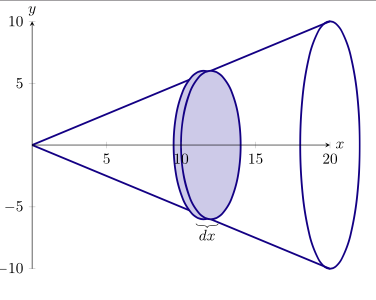
\includegraphics [scale=0.4] {cone_sideways.png}\end{center}
The cone is three-dimensional with the third axis ($z$) coming up out of the page.  The intersection with the $xy$-plane is a triangle.  

Can you see that in the $xy$-plane $y$ is a linear function of $x$, i.e. $y = kx$ where $k$ is a constant.  (The constant $k$ is actually the ratio of the radius $R$ to the height $H$.  That is equal to $\Delta y/\Delta x$.).
\[ y = \frac{R}{H} x \]

If we slice the cone into thin sections perpendicular to the $x$-axis, each little piece is a circle with radius $y$ and area $\pi y^2$.  For a thin enough slice, the volume is that area times the width of the slice:
\[ dV = \pi y^2 \ dx \]
Finding the volume of an individual piece is the important part of the calculus argument.

Now we just substitute the value of $y$ in terms of $x$
\[ dV = \pi \ [ \frac{R}{H} ]^2  x^2 \ dx \]
add up all the little volumes by setting up the integral
\[ V = \int dV = \int \pi \ [ \frac{R}{H} ]^2 x^2 \ dx \]

We apply a basic rule that constant terms can move "out from under" the integral sign:
\[ = \pi \ [ \frac{R}{H} ]^2 \ \int x^2 \ dx \]

We recognize that the value $x$ lies in the interval $[0,H]$ so these are the "bounds" on the integral
\[ = \pi \ [ \frac{R}{H} ]^2 \int_0^H x^2 \ dx \]

and then just follow the rule for doing a problem like this:  $\int x^2 = x^3/3$.  So
\[ = \pi \ [ \frac{R}{H} ]^2 \ [  \frac{x^3}{3} ] \ \bigg |_0^H \]
\[ = \frac{1}{3} \pi R^2 H \]

Once again, we obtain the formula of one-third times the area of the base times the height.  No matter what the shape of the base is, the area of each slice will be proportional to $x^2$ and we will end up with a formula involving one-third at the end.

We will see several other methods for obtaining this result.

We also note that we can obtain the volume of a fustrum (look it up) as
\[ = \pi \ [ \frac{R}{H} ]^2 \ [  \frac{x^3}{3} ] \ \bigg |_{h_1}^{h_2} \]
\[ = \pi \ [ \frac{R}{H} ]^2 \ [  \frac{{h_2}^3}{3} -  \frac{{h_1}^3}{3}  \ ] \]


\end{document}